\chapter[Justificativa]{Justificativa}
O Brasil tem um dos piores índices de conhecimento em matemática \cite{indiceRuimMat}. Também tem o desânimo dos alunos e professores além da falta de estratégias inovadores por parte dos professores na hora de ensinar \cite{softwaregamificado}. Esse método de ensino tradicional, onde o professor é ativo e os alunos são apenas passivos para receber o conhecimento faz com que menos seja abstraído pelos alunos, que também precisam de práticas e um tempo de ócio criativo para abstrair e compreender o conteúdo de modo a repetir e aplicar em outras situações. Pouco foi-se encontrado de estudos na área de \textbf{matemática} + \textbf{gamificação}. A quantidade de estudos diminui quando o conteúdo de matemática é do ensino superior ao invés de ensino de matemática no ensino fundamental. 
Um outro problema é a falta de inclusão de alunos com necessidades especiais nos ambientes de sala de aula, isso deve-se à falta de preparo dos professores em sua formação \cite{matEtdah}.
Não foi encontrado nenhum jogo de matemática para o ensino e/ou suporte de EDO. Apenas um jogo de vídeo-game que aplica ED na movimentação dos personagens (princípio da dinâmica de Newton)\cite{videoGameED}.
Avaliou-se o índice de reprovação na disciplina Cálculo 2 (C2) na UnB, nos semestres 2/2017 e 1/2018. A média foi a seguinte:

\begin{table}[H]
\centering
\caption{Percentual de reprovações no semestre 2/2017 e 1/2018}
\begin{tabular}{|c|c|c|}
\hline
Semestre & Total de menções & Percentual de reprovados \\ 
\toprule
2/2017 & 1164 & 32.47\% \\ 
1/2018 & 1101 & 31.88\% \\
\textbf{Total} & 2265 & 32.18\% \\
\hline
\end{tabular}
\label{tabelareprovacaoC2}
\small{Fonte: do próprio autor}
\end{table} 

A tabela mostra que aproximadamente 32\% dos alunos reprovaram de um total de 2265 alunos. 
A figura \ref{figuramencao} é um gráfico de pizza, mostra o percentual médio das menções dos alunos da UnB de C2 nos períodos de 2/2017 e 1/2018.

\begin{figure}[H]
\centering
\caption{Percentual das menções de C2 em 2/2017 e 1/2018}
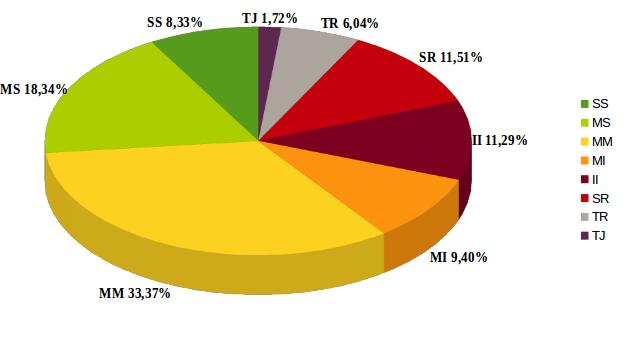
\includegraphics[scale=0.72]{figuras/grafico_media.jpg}
\label{figuramencao}
\small{Fonte: do próprio autor}
\end{figure}

O desenvolvimento do jogo é para os alunos terem uma ferramenta a mais como meio de treinamento e fixação do conhecimento para aumentarem suas menções, tendo em vista que a maior parte das menções está concentrada na menção MM, com aproximadamente 33\%. O percentual de MS é aproximadamente 18\% e SS próximo de 8\%.

No primeiro semestre de 2019, 
Serão aplicados questionários e recebidos os dados estatísticos do jogo que só poderão ser recebidos quando os usuários enviarem. 